
\section{Histogram \cite{ism-2, wiki-histogram}}\label{histogram}
\subsection{Constructing a Histogram for Discrete Data}
\begin{enumerate}
    \item determine the frequency and relative frequency of each x value
    \item mark possible x values on a horizontal scale
    \item Above each x value, draw a rectangle whose height is the relative frequency (or alternatively, the frequency) of that value
\end{enumerate}

\subsection{Constructing a Histogram for Continuous Data: Equal Class Widths}
\begin{enumerate}
    \item Determine the frequency and relative frequency for each class.
    \item Mark the class boundaries on a horizontal measurement axis.
    \item Above each class interval, draw a rectangle whose height is the corresponding relative frequency (or frequency).
\end{enumerate}

\subsection{Constructing a Histogram for Continuous Data: Unequal Class Widths}
\begin{enumerate}
    \item After determining frequencies and relative frequencies, calculate the height of each rectangle using the formula:
    \begin{equation}
        (rectangle\_height) = (relative\_frequency\_of\_the\_class) / (class\_width)
    \end{equation}
    \item The resulting rectangle heights are usually called \textbf{densities}\indexlabel{densities (histogram)}, and the vertical scale is the density scale. 
    \item This prescription will also work when class widths are equal. 
    \item the area of each rectangle is proportional to the relative frequency of the value
\end{enumerate}

\begin{table}[H]
    \begin{minipage}{0.45\textwidth}
        \centering
        \begin{tabular}{|c|c|}
            \hline
            Bin/Interval & Count/Frequency \\ \hline
            -3.5 to -2.51 & 9 \\ \hline
            -2.5 to -1.51 & 32 \\ \hline
            -1.5 to -0.51 & 109 \\ \hline
            -0.5 to 0.49 & 180 \\ \hline
            0.5 to 1.49 & 132 \\ \hline
            1.5 to 2.49 & 34 \\ \hline
            2.5 to 3.49 & 4 \\ \hline
        \end{tabular}
        \caption{Data: Histogram}
    \end{minipage}
    \hfill
    \begin{minipage}{0.45\textwidth}
        \begin{figure}[H]
            \centering
            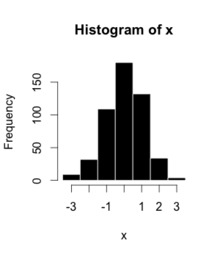
\includegraphics[height=5cm]{Pictures/data/data_histogram.jpg}
            \caption{Graph: Histogram}
        \end{figure}
    \end{minipage}
\end{table}


